\section{Data}
\label{app:data}
\paragraph{Nemo-Gym.}~\citep{nemogym}
We selected four heterogeneous tasks served from the NeMo-Gym servers, some requiring tool-use or multi-turn capabilities, some do not.
\textbf{\texttt{IF}} draws its training prompts from the WildChat-1M dataset~\citep{zhao2024wildchat1mchatgptinteraction} with instructions from the Open-Instruct code base~\citep{ahmad2025opencodeinstructlargescaleinstructiontuning}, and is evaluated on the held-out IF-Bench~\citep{ifbench}. \textbf{\texttt{code\_gen}} contains competitive coding challenges from
NVIDIA's OpenCodeReasoning~\citep{ahmad2025opencodereasoningadvancingdatadistillation} dataset. This dataset is served with Nemo-Gym's single-turn verification engine \texttt{code\_gen}.
\textbf{\texttt{xlam\_fc}}~\citep{zhang2024xlamfamilylargeaction} is an API/function calling dataset in xLAM format.
\textbf{\texttt{workplace}}~\citep{nemogym} is a tool-use multi-step agentic environment that tests the agent’s ability to execute tasks in a workplace setting such as calendar scheduling or email management.
Tab.~\ref{tab:agentic} lists the per-task train and test sizes.


\paragraph{Reasoning-Gym.}~\citep{reasoninggym}
Our reasoning mixture is procedurally generated with scripts offered by Reasoning-Gym~\citep{reasoninggym}.
Each task is instantiated at three difficulty levels (easy, medium, and hard) with 30000 training and 600 test problems. We describe the individual tasks below.
\textbf{\texttt{ARC-1D}} is an abstract pattern-induction puzzle where the agent infers the grid transformation rule from examples.
\textbf{\texttt{countdown}} is a numbers game in which the agent combines given numbers and fixed set of operations to hit a target.
\textbf{\texttt{zebra}} a logic game where you use clues and deduction to match attributes across different colored houses.
\textbf{\texttt{word\_sorting}} is an alphabetical word-sorting task.
In \textbf{\texttt{puzzle24}}, one needs to combine four numbers and basic arithmetic operations to make 24. 
In \textbf{\texttt{manipulate\_matrix}}, one must apply given grid operations in sequence to reach a given state.
App.~\ref{app:rg-generation} reports the complete generation configurations.

\begin{table}[t]
\centering
\small
\setlength{\tabcolsep}{8pt}
\begin{tabular}{@{}llrrl@{}}
\toprule
Task & Capability & \# Train & \# Test & Test set \\
\midrule
instruction\_following & constraint following   & 45891 & 300 & \textbf{IF-Bench} (held out) \\
code\_gen              & program synthesis      & 23971 & 322 & in-distribution \\
xlam\_fc               & function / tool calling& 59000 & 1000& in-distribution \\
workplace\_assistant   & multi-turn assistant   & 1255  & 545 & in-distribution \\
\bottomrule
\end{tabular}
\caption{Agentic multi-task suite. Instruction following is trained on a constraint-following
pool and evaluated on the held-out IF-Bench benchmark; the other three tasks use in-distribution
test splits. Sizes are the number of served problems.}
\label{tab:agentic}
\end{table}

\subsection{Reasoning-Gym Data Generation}
\label{app:rg-generation}

All six reasoning tasks are generated procedurally with Reasoning-Gym~\citep{reasoninggym}
using a single builder that fixes the prompt template, answer schema, difficulty schedule, and
random seeding, so every instance is fully reproducible and paired with a deterministic,
rule-based verifier.

\paragraph{Difficulty control.}
Difficulty is set at generation time through each task's generator configuration rather than by
post-hoc filtering. Five tasks are produced at three levels---\emph{easy}, \emph{medium}, and
\emph{hard}---and \texttt{puzzle24} is produced as a single un-tiered level (its curriculum is
degenerate). The controlling knob per task is:
\begin{itemize}
  \item \textbf{\texttt{word\_sorting}}: the Reasoning-Gym \texttt{WordSortingCurriculum} global level
        ($0/1/2$ for easy/medium/hard) under upper-bound range semantics, which widens the
        number-of-words and word-length ranges as difficulty increases.
  \item \textbf{\texttt{manipulate\_matrix}}: a fixed $10{\times}10$ integer grid with the number of chained
        transformations set to $1/3/5$ for easy/medium/hard. We scale difficulty by transformation
        \emph{depth} rather than grid size, because larger grids inflate the target answer beyond
        the response-length budget.
  \item \textbf{\texttt{puzzle24}}: the generator default. The operand values, $[1,10]$, are evenly split between three difficulty levels.
  \item \textbf{\texttt{arc}}, \textbf{\texttt{countdown}}, \textbf{\texttt{zebra}}: 
These three families are drawn from Reasoning-Gym's procedural generators under their built-in
difficulty \emph{curricula}, whose discrete levels the easy/medium/hard tiers index. \emph{Countdown} presents a multiset
of source integers to be combined with $+,-,\times,\div$ into a target. Its
\texttt{CountdownCurriculum} sets difficulty through three range attributes: the operand count
(level ladder $\{3,6,9,12,15\}$), the target magnitude ($\{100,500,1000,5000,10000\}$), and the
source-value magnitude ($\{1,100,200,300\}$). Harder tiers grant more operands and larger targets and values. \emph{Zebra} is an Einstein-style constraint-satisfaction puzzle. Its
\texttt{ZebraPuzzleCurriculum} scales two attributes, the number of people and the number of characteristics, each over $\{2,\dots,7\}$, enlarging the constraint grid as difficulty rises.
\emph{ARC} draws ARC-AGI-1 grid-transformation tasks and raises difficulty through two
augmentation-weight distributions: a rotation distribution over
$\{\text{identity},90^\circ,180^\circ,270^\circ\}$, shifted from identity-dominant
($[0.3,0.2,0.3,0.2]$) toward rotation-dominant ($[0.0,0.4,0.2,0.4]$), and a mirror distribution over
$\{\text{identity},\text{horizontal},\text{vertical},\text{diagonal},\text{counter-diagonal}\}$,
shifted from simple toward diagonal mirrors ($[0.3,0.3,0.2,0.1,0.1]\!\rightarrow\![0.05,0.05,0.1,0.4,0.4]$).
All three inherit the per-instance seeding, three-tier schedule, and \verb|\boxed{}| answer schema of
the other tasks.
\end{itemize}


\section{Concavity Test}
\label{app:concavity}

\begin{figure}[t]
  \centering
  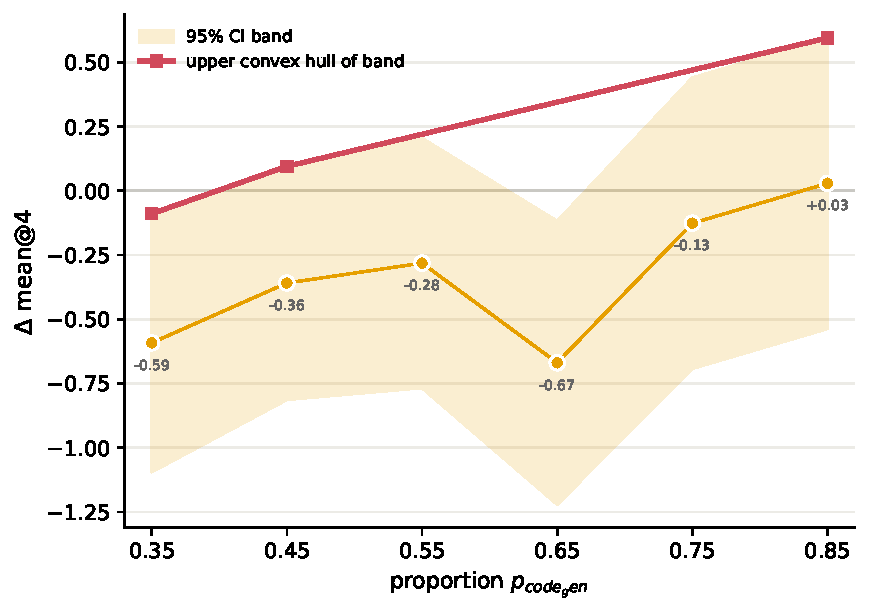
\includegraphics[width=0.48\textwidth]{fig/probe_code_gen_upperhull.pdf}\hfill
  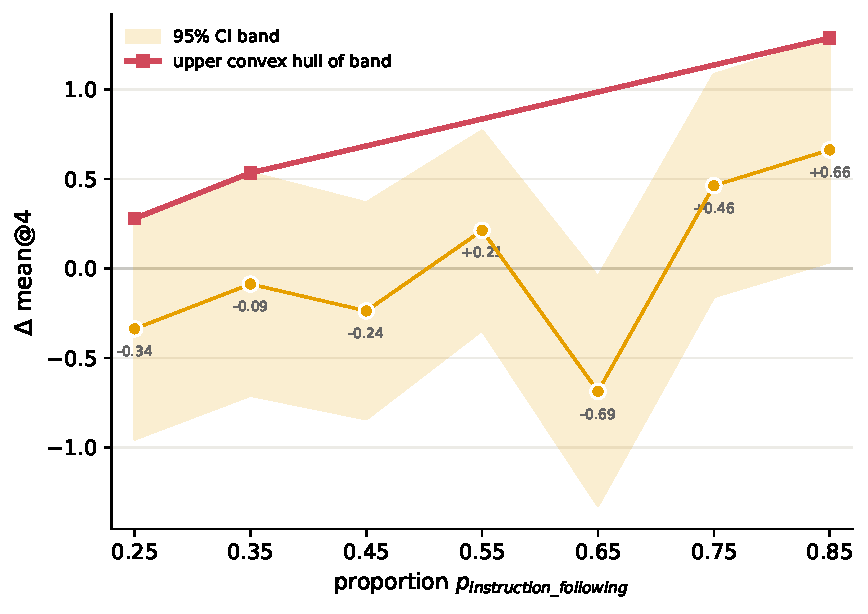
\includegraphics[width=0.48\textwidth]{fig/probe_IF_upperhull.pdf}\\[0.6em]
  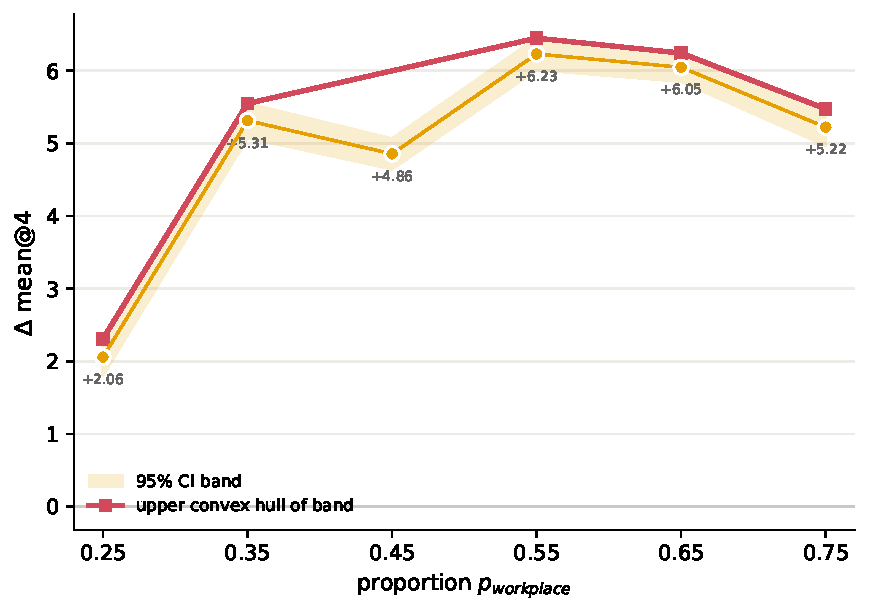
\includegraphics[width=0.48\textwidth]{fig/probe_workplace_upperhull.pdf}\hfill
  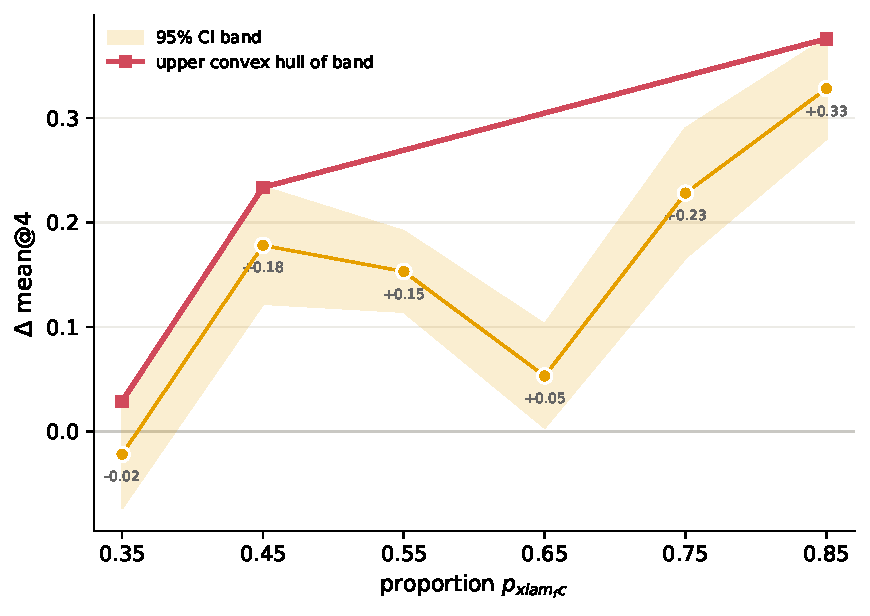
\includegraphics[width=0.48\textwidth]{fig/probe_xlam_upperhull.pdf}
  \caption{\textbf{Allocation response of each Nemo-Gym task.} Change in mean@4 after $10$
  steps from a common step-$80$ checkpoint, as the probed task's share of the batch is swept
  from $0.25$ to $0.85$ and the remaining mass is split evenly among the other three tasks.
  Shaded region is the $95\%$ confidence band; the upper curve is its upper convex hull, the
  tightest concave envelope the measurements admit.}
  \label{fig:concavity_probe}
\end{figure}

\Cref{asm:concavity} asks only that task improvement respond concavely to allocation, and we
check this directly rather than assume it. Starting from a common step-$80$ checkpoint of the
four-task Nemo-Gym run, we probe one task at a time: its share is held at one of seven values
from $0.25$ to $0.85$ in steps of $0.10$, the remaining budget is split evenly among the other
three tasks, and training continues for $10$ steps. Each probe is scored by the change in
mean@4 from the checkpoint, and repeated sampling gives the $95\%$ confidence band shown in
\Cref{fig:concavity_probe}, against which we run an upper-convex-hull test for concavity. All
four tasks display a concave trend over the probed range, which supports
\Cref{asm:concavity} as a working assumption for this setting. The probe covers one checkpoint
and one mixture, so it speaks to local rather than global concavity of the task-improvement
surface.


\section{Diagonal-Jacobian PDCM}
\label{app:diagonal}

% Diagonal-Jacobian ablation. Totals verified against the per-task numbers.
\begin{table}[t]
\centering
\caption{Full versus diagonal Jacobian in \textsc{PDCM}, on the four Nemo-Gym tasks.
\textsc{PDCM} estimates the full allocation-response Jacobian $G_t$;
\textsc{PDCM}$_{\mathrm{diag}}$ keeps only its diagonal, treating each task's improvement as a
univariate function $\widehat U_{t,k}(p_{t,k})$ of its own share (\Cref{app:diagonal});
Uniform is the even-split baseline. Best per task in \textbf{bold}, second best
\underline{underlined}.}
\vspace{-0.1in}
\label{tab:diag-ablation}
\setlength{\tabcolsep}{3.4pt}
\renewcommand{\arraystretch}{1.12}
\resizebox{0.72\textwidth}{!}{%
\begin{tabular}{l ccc c ccc}
\toprule
 & \multicolumn{3}{c}{\textbf{pass@1}} & & \multicolumn{3}{c}{\textbf{pass@4}} \\
\cmidrule(lr){2-4} \cmidrule(lr){6-8}
Task & PDCM & PDCM$_{\mathrm{diag}}$ & Uniform & & PDCM & PDCM$_{\mathrm{diag}}$ & Uniform \\
\midrule
code\_gen  & 32.61 & \textbf{35.09} & \underline{34.08} & & 40.55 & \textbf{43.50} & \underline{41.41} \\
IF         & \underline{53.33} & \textbf{53.92} & 47.58 & & \textbf{61.21} & \underline{60.38} & 54.57 \\
workplace  & \textbf{82.89} & 79.86 & \underline{81.74} & & \textbf{88.15} & 83.35 & \underline{84.00} \\
xlam       & \textbf{84.35} & \underline{83.95} & 74.87 & & \textbf{84.66} & \underline{84.28} & 80.70 \\
\midrule
Total      & \textbf{253.18} & \underline{252.82} & 238.27 & & \textbf{274.57} & \underline{271.51} & 260.68 \\
\bottomrule
\vspace{-\intextsep}
\end{tabular}}
\end{table}


\Cref{alg:pdcm_jacobian} estimates the full allocation-response Jacobian $G_t$, whose entry
$g_{t,kj}$ records how task $k$'s improvement responds to task $j$'s share of the batch. A
simpler variant keeps only the diagonal. It is worth setting out on its own, both because it is
the regime in which our theoretical results are stated and because it is the variant whose
signal we can estimate most reliably.

The restriction amounts to assuming that each task's improvement depends on the allocation only
through that task's own share,
\begin{equation}
U_{t,k}(p) \;=\; U_{t,k}(p_k), \qquad k\in[K],
\label{eq:separable-utility}
\end{equation}
so the aggregate utility $U_t(p)=\sum_{k=1}^K U_{t,k}(p_k)$ is separable and each $U_{t,k}$ is a
\emph{univariate} function of $p_k$ alone. This is exactly the object the estimator of
\Cref{eq:policy_improvement_estimation} measures: $\widehat U_{t,k}$ is read off the rollouts
that task $k$ received under its own share $p_{t,k}$, so the empirical quantity the controller
actually observes is $\widehat U_{t,k}(p_{t,k})$, a scalar response to a scalar input. Under
\Cref{eq:separable-utility} the supergradient of \Cref{asm:concavity} has a single nonzero
coordinate, $g_{t,k}=U_{t,k}'(p_{t,k})\,e_k$, and $G_t$ collapses to
$\operatorname{diag}(g_{t,11},\ldots,g_{t,KK})$ with $g_{t,kk}=U_{t,k}'(p_{t,k})$.

Three parts of the algorithm simplify accordingly. The score of
\Cref{eq:dual_weighted_marginal_utility_vectorized} loses its cross terms and becomes
coordinatewise,
\begin{equation}
s_{t,k} \;=\; \bigl(1+\lambda_{t,k}\bigr)\, g_{t,kk},
\label{eq:diag-score}
\end{equation}
so each task's score is its own marginal utility amplified by its own lag pressure, and budget
reaches a lagging task only by being withdrawn from the others through the simplex rather than
by exploiting cross-task transfer. The lag certificate reduces from an inner product to a
product of scalars, $\langle g_{t,k},u-p_t\rangle = g_{t,kk}\,(u-p_{t,k})$, and the dual update
of \Cref{eq:dual_update} follows unchanged. Finally, curvature estimation
(\Cref{sec:curv_est}) reduces from $K^2$ entries to $K$: the Theil--Sen regression of
\Cref{eq:theil-sen} is run once per task over the pairs
$\{(p_{\tau,k},\widehat U_{\tau,k})\}_{\tau=t-H}^{t-1}$, and needs only variation in a task's
own share rather than independent variation in every coordinate of $p$.

The trade-off is that the diagonal variant cannot represent transfer: if training on task $j$
raises task $k$'s return through shared parameters, that effect is invisible to
\Cref{eq:diag-score} and is absorbed into the drift of $U_{t,k}$ over rounds. What it buys is
conditioning. Identifying the off-diagonal entries requires the allocation to vary
independently along every coordinate, which the controller does not deliberately produce, and
the number of entries grows as $K^2$ while each task's share shrinks as $1/K$ --- the same
pressure discussed in \Cref{sec:scaling}. The diagonal entries, by contrast, are identified by
precisely the variation the primal update generates on its own. The probe of
\Cref{app:concavity} measures this univariate response directly, sweeping $p_{t,k}$ with the
remaining mass held even, and is therefore a test of \Cref{asm:concavity} in exactly the
diagonal form used by \Cref{thm:no-regret}.

\Cref{tab:diag-ablation} compares the two variants on the four Nemo-Gym tasks. Both clear the
uniform baseline comfortably, and their totals are close: the diagonal variant trails the full
Jacobian by $0.36$ points at pass@1 and $3.06$ at pass@4. The per-task pattern is more
informative than the totals. $\texttt{PDCM}_{\mathrm{diag}}$ is the stronger of the two on
$\texttt{code\_gen}$ at both metrics and edges ahead on $\texttt{IF}$ at pass@1, but it gives up
$3.03$ points on $\texttt{workplace}$ at pass@1 and $4.80$ at pass@4, the task whose gains the
full Jacobian attributes most strongly to allocation elsewhere in the mixture. Discarding the
off-diagonal entries therefore costs little in aggregate while removing the mechanism by which
one task's budget is credited with another's improvement.
